
\section{Rozpoznávanie a klasifikácia}
\label{sec:klasifikacia}

%\# TODO - dopisať čo je to Klasifikácia

\subsection{K-Nearest-Neighbor}
\textit{k}-Nearest Neighbor je algoritmus, ktorý sa učí pod dozorom [eng. supervised learning algorithm] často používaný pri rozpoznávaní vzorov v klasifikácií,
avšak je možné ho použiť aj pre odhad a predikciu\cite{book:DataMining}.
Algoritmus je pamäťovo náročný [eng. memory-based] a nepotrebuje žiaden trénovací model.
Pre jeho fungovanie nie je potrebný žiaden explicitný postup trénovania, okrem zberu vektorov príznakov s označeniami tried do ktorých patria.

Klasifikácia dát prebieha v 2 krokoch: nájdenie \textit{k} najbližších susedov spomedzi trénovaných dát a
vykonanie ''väčšinové hlasovanie'' medzi nájdenými susedmi pre priradenie najčastejšie sa vykytovaného označenia triedy.

Nech $\{ (x_i, y_i); i = 1, 2, \dots, n \}$ je množína trénovacích dát, kde $x_i$ je vektor príznakov a $y_i$ je názov triedy do ktorej patrí vektor $x_i$.
Predpokladáme že každé $x_i$ je v určitom multidimenzionálnom priestore príznakov s metrikov $P$ a $y_i \in \{ 1, 2, \dots, l \}$, kde $y_i$ je číslo odpovedajúcej triedy.
Cieľom je priradiť neoznačeny vektor $x$ do zodpovedajucej triedy z množiny $\{ 1, 2, \dots, l \}$.

Najjednoduchšia verzia algoritmu \textit{k}-NN je 1-NN, kde vektor $x$ je priradený najbližsiemu susedovi.
To znamená že ak $x_j$, kde $j \in \{ 1, 2, \dots, n \}$, je najbližšií k $x$ vo forme vzdialenosti $P$ \cite{prop:KnnClassification}:
\begin{equation}
    \label{eq:kNNMetric}
    x_j = arg \; min_{\{x_i, 1 \leq i \leq n\}} P(x, x_i)
\end{equation}
tak označenie triedy pre vektor $x$ je číslo $y_i$.

Pre formu algoritmu \textit{k}-NN, kde $k > 1$ je postup podobný, ale priradenie označenia triedy pre $x$ je na základe najčastejšie sa vyskytovaného označenia triedy
spomedzi \textit{k} najbližších susedov z trénovacích bodov $x_i$, kde $k$ je užívateľom definovaná konštanta \cite{prop:KnnClassification}.

Najbežnejší výpočet pre vzdielenosť bodov je pomocou Euklidovskej vzdielenosti.
Táto vzdielnosť je medzi dvoma $J$-dimenzionálnymi vektormi $a$ a $b$ vyjadrená ako \cite{prop:KnnClassification}:
\begin{equation}
    \label{eq:euclidMetric}
    d_{a,b} = \sqrt{\sum_{j=1}^{J}{(a_j - b_j)^2}}
\end{equation}

Na obrázku \ref{pic:kNN} je zobrazený rozdiel medzi 1-NN a 5-NN algoritmom pre klasifikáciou,
    použitím 2-dimenzionálnych bodov a 3 tried dát (červená, modrá, zelená).
Farebné regióny vyznačujú rozhodovacie hranice klasifikátora, ktorý využíva Euklidovskú vzdielnosť.
Biele oblasti ukazujú body, ktoré sú nejednoznačne klasifikované (to znamená, že hodnotenie triedy je viazané aspoň na dve triedy).
V ukážke je vidno že v prípade 1-NN klasifikátora, niektré body vytvárajú ''malé ostrovy''
    (napr. zelený bod v strede mraku medzi modrými bodmi), zatiaľ čo 5-NN klasifikátor vyhladzuje tieto nezrovnalosti,
    a pravdepodobne vedie k lepšiemu zovšeobecneniu nad testovacími údajmi.

\begin{figure}[H]
	\centering
	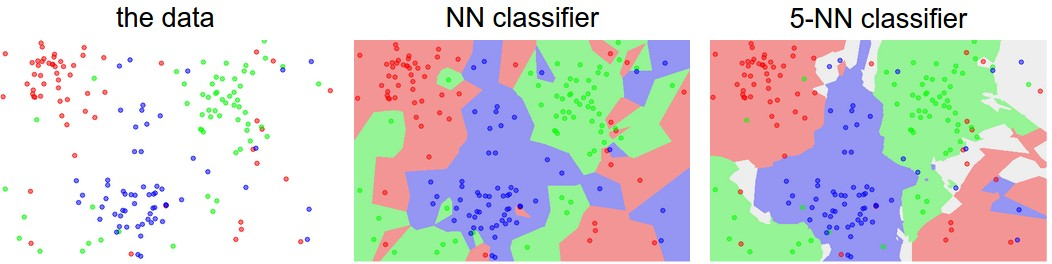
\includegraphics[width=1\textwidth]{knn}
	\caption{Porovnanie k-NN klasifikátorov\cite{odkaz:KnnImage}}
	\label{pic:kNN}
\end{figure}


\subsection{Support Vector Machines}
Support Vector Machines (SVM's) sú metódy učenia používané pre binárnu klasifikáciu.
Základnou myšlienkou je nájdenie hyper--roviny, ktorá perfektne oddelí \textit{d}--dimenzionálne dáta do dvoch tried\cite{prop:IntroductionToSVM}.
SVM sa snaží maximalizovať vzdialenosť medzi rozdeľujúcou rovinou a dátami nachádzajúcimi sa v každej z 2 polrovín\cite{prop:SupervisedMachineLearning}.
Avšak kedže vstupné dáta väčšinou nie su lineárne separovatelné, SVM's predstavujú pojem “kernel induced feature space”,
    ktorý prevádza dáta do vyššieho dimenzionálneho priestoru, kde sú dáta oddeliteľné.\cite{prop:IntroductionToSVM}

Ak trénovacie dáta sú lineárne separovatelné, tak dvojica $(w, b)$ existuje ako\cite{prop:SupervisedMachineLearning}:
\begin{equation}
    \label{eq:SVMPair1}
    w^T * x_i + b \geq 1, \; pre \; x_i \in P
\end{equation}
\begin{equation}
    \label{eq:SVMPair2}
    w^T * x_i + b \leq -1, \; pre \; x_i \in N
\end{equation}
s rozhodovacím pravidlom
\begin{equation}
    \label{eq:SVMDecisionRule}
    f_{w,b}(x) = sgn(w^T x + b)
\end{equation}
kde $w$ je váhový vektor a $b$ je predpoveď (alebo $-b$ je prahová hodnota).
V tomto prípade keď je možné lineárne rozdeliť dve triedy, tak optimálna hyper--rovina pre rozdelenie
    môže byť nájdena, minimalizáciou kvadratickej formy rozdeľujúcej hyper--roviny
\begin{equation}
    \label{eq:SVMDecisionRule}
    mininimize_{w,h} \; \Phi(w) = \frac{1}{2}||w||^2, \; pre \; y_i(w^Tx_i + b) \geq 1, i = 1, \dots, l
\end{equation}

V tomto prípade lineárneho rozdelenia dát, pri nájdení optimálnej rozdeľujúcej hyper--roviny, dátove body, ktoré ležia na jej okraji
    sa nazývajú podporné vektorové body[eng. support vector points] a riešenie je reprezentované ako lineárna kombinácia iba 3 týchto bodov (vid. obrázok \ref{pic:SVMMAxMargin} ).
Ostatné body sú ignorované\cite{prop:SupervisedMachineLearning}.

\begin{figure}[H]
	\centering
	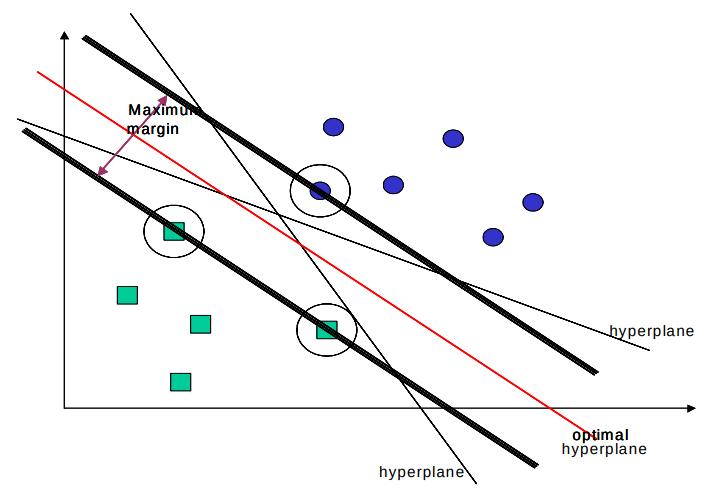
\includegraphics[width=1\textwidth]{SVM_max_margin}
	\caption{Maximálne rozpätie\cite{prop:SupervisedMachineLearning}}
	\label{pic:SVMMAxMargin}
\end{figure}

Avšak väčsina reálnych problémou zahŕňa nelineárne rozdelenie dát pre ktoré neexistuje žiadna hyper--rovina, ktorá by úspešne rozdelila trénovacie dáta.
Riešenie tohto problému je mapovať dáta do vyššie--dimenzionálneho priestoru a definovať tam rozdeľujúcu hyper--rovinu.
Tento vyššíe-dimenzionálny priestor je tzv. transformovaný priestor príznakov[eng. transformed feature space], ako opak ku vstupnému priestoru[eng. input space] obsahujúcemu trénovacie dáta\cite{prop:SupervisedMachineLearning}.

Pri vhodne zvolenom transformovanom priestore príznakov dostatočnej veľkosti, môžu byť všetky trénovacie dáta rozdelitelné.
Lineárne rozdelenie v tomto priestore zodpovedá nelineárnemu rozdeleniu v pôvodnom vstupnom priestore.

Pri mapovaní dát do určitého Hilbertovho priestora \cite{prop:HilbertSpace} $H$ ako $\Phi:R^d \rightarrow H$.
Potom trénovací algoritmus závisý len na údajoch zo skalárneho súčinu[eng. dot products] v priestore $H$, t.j na funkciách v tvare $\Phi(x_i) * \Phi(x_j)$.
Ak bude existovať ''funkcia jadra''[eng. kernel function] $K$ ako $K(x_i, x_j) = \Phi(x_i)*\Phi(x_j)$, tak budeme musieť použiť iba funkciu $K$ v trénovacom algoritme
    a nikdy nebudeme potrebovať explicitne definovať $\Phi$\cite{prop:SupervisedMachineLearning}.

Takže jadrá[eng. kernels] sú špeciálnou triedou funkcií, ktoré dovoľujú, aby sa vnútorné produkty vypočítali priamo vo funkčnom priestore[eng. feature space] bez toho, aby sa vykonalo vyššie popísané mapovanie.
Po vytvorení hyper--roviny sa funkcia jadra použije na mapovanie nových bodov do funkčného priestoru pre klasifikáciu\cite{prop:SupervisedMachineLearning}.

Voľba správnej funkcie jadra je veľmi dôležitá, kedže definujú transformovaný priestor príznakov v ktorom budú trénovacie dáta klasifikované.
Genton \cite{prop:KernelClasses} popísal niekoľko tried jadier, avšak, neadresoval otázku, ktorá trieda je najvhodnejšie pre daný problém.

Zoznam populárnych jadier\cite{prop:SupervisedMachineLearning}:
\begin{equation}
    K(x, y) = (x*y+1)^P
\end{equation}
\begin{equation}
    K(x, y) = e^{\frac{-||x-y||^2}{2 \sigma^2}}
\end{equation}
\begin{equation}
    K(x, y) = tanh(\kappa x*y - \delta)^P
\end{equation}

\begin{figure}[H]
	\centering
	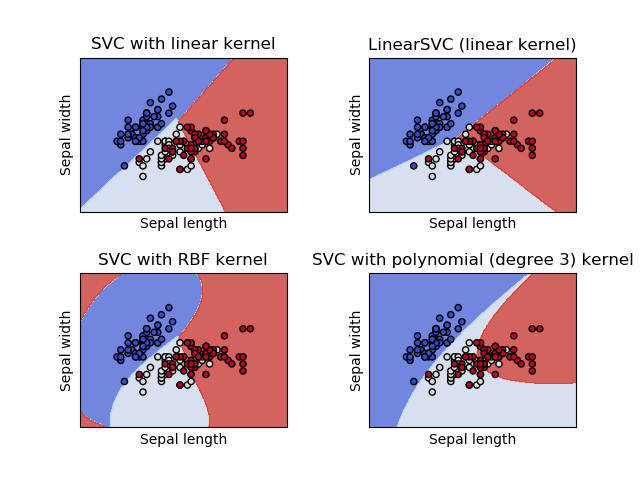
\includegraphics[width=1\textwidth]{sphx_glr_plot_iris_0012}
	\caption{Porovnanie rôznych typov SVM klasifikátorov\cite{odkaz:SVMImage}}
	\label{pic:SVMComparison}
\end{figure}


\subsection{Stochastic Gradient Descent}
Výpočtova zložitosť algoritmov učenia sa stáva kritickým obmedzujúcim faktorom, pri používaní veľmi rozsiahlých množín vstupným dát.
Preto sa pre veľké množiny dát začal používať Stochastic Gradient Descent\cite{prop:StochasticGradientDescent}, ktorý tieto výpočty dokáže optimalizovať.

Každý vzor $z$ je pár $(x, y)$ kde $x$ je ľubovolný vstup a $y$ skalárny výstup.
Máme stratovú funkciu [eng. loss function] $\ell(\hat{y},y)$ ktorá meria hodnotu predpovedania $\hat{y}$ keď správna odpoveď je $y$,
    a zvolíme si rodinu $\mathcal{F}$ funkcií $f_w(x)$ parametrizované váhovym vektorom $w$.

Hľadáme funkciue $f \in \mathcal{F}$, ktorá minimalizuje stratu $Q(z,w) = \ell(f_w(x), y)$ spriemerovanú vzhľaďom na vzory $z$.
Avšak pre napodobenie prírody je prirodzenejšie priemerovať vzhľadom na neznámu distribúciu $dP(z)$\cite{prop:StochasticGradientDescent}.
\begin{equation}
    E(f) = \int{\ell(f(x), y)dP(z)} \quad E_n(f) = \frac{1}{n}\sum_{i=1}^{n}\ell(f(x_i), y_i)
\end{equation}
$E_n(f)$ meria výkonnosť trénovacích dát. $E(f)$ meria generalizovanú výkonnosť, teda očakávaný výkon v budúcich vzorkách.

Pomocou klesania gradientu[eng. gradient descent] minimalizujeme $E_n(f_w)$, kde každá iterácia aktualizuje váhove vektory $w$ na základne gradientu.
\begin{equation}
    w_{t+1} = w_t - \gamma \frac{1}{n}\sum_{i=1}^{n}\bigtriangledown_w Q(z_i, w_t)
\end{equation}
kde $\gamma$ je vhodne zvolený zisk[eng. gain].

Stochastic Gradient Descent algoritmus je drastické zjednodušenie.
Namiesto počítania gradientu pre $E_n(f_n)$, každá iterácia odhadne tento gradient na základe jednej náhodne vybranej vzorky $z_t$\cite{prop:StochasticGradientDescent}:
\begin{equation}
    w_{t+1} = w_t - \gamma \bigtriangledown_w Q(z_t, w_t)
\end{equation}


\subsection{Neurónové siete}
Neurónová sieť (NN) je masívne paralelný procesor, ktorý má sklon k uchovávaniu experimentálnych znalostí a ich ďalšieho využívania.
Napodobňuje ľudský mozog v dvoch aspektoch \cite{odkaz:NNIntroduction}:
\begin{enumerate}
	\item[$\bullet$] poznatky sú zbierané v NN počas učenia
	\item[$\bullet$] medzineurónové spojenia (synaptické váhy - SV) sú využívané na ukladanie znalostí
\end{enumerate}
Toto je jedna z definícii NN, akceptovaná NN komunitou.
Je zrejmé, že inšpirácia ku vzniku NN prišla z biologických systémov.
Na prvý dojem vysoko abstraktná disciplína nachádza množstvo aplikácii v praxi a stáva sa prostriedkom pre riešenie problémou v širokom spektre odborných oblastí\cite{odkaz:NNIntroduction}.

Rôzne architektúry umelých neurónových sieti[eng. artificial neural network] sa používajú pre riešenie rôznych úloh.
Konvolučné a rekurentné NN sú dve z najúspešnejších a sú z veľkej časti zodpovedné za nedávnu revolúciu umelej inteligencie\cite{odkaz:CorrectionOfImageOrentation}.

Vo všeobecnosti môžeme vymenovať nasledovné oblasti využitia neurónových sieti\cite{odkaz:NNIntroduction}:
\begin{enumerate}
    \item[$\bullet$] klasifikácie do tried, klasifikácia situácií
    \item[$\bullet$] riešenie predikčných problémou
    \item[$\bullet$] problémy riadenia procesov
    \item[$\bullet$] tranformácia signálov
\end{enumerate}

Neurónové siete sú usporiadané do vnútorne prepojených vrstiev umelých neurónov.
Jednoducho povedané, každá vrstva berie výstup z prechádzajucej vrstvy, aplikuje transformácie a výsledok pošle na vstup ďalšej vrstve.
Prvá vrstva vstupov je prepojená na vstupné dáta, ktoré sa majú spracovať a posledná vrstva je akýkoľvek výstup, ktorý chceme predpovedať \cite{odkaz:CorrectionOfImageOrentation} (vid. obrázok \ref{pic:NNExample}).
\begin{figure}[H]
	\centering
	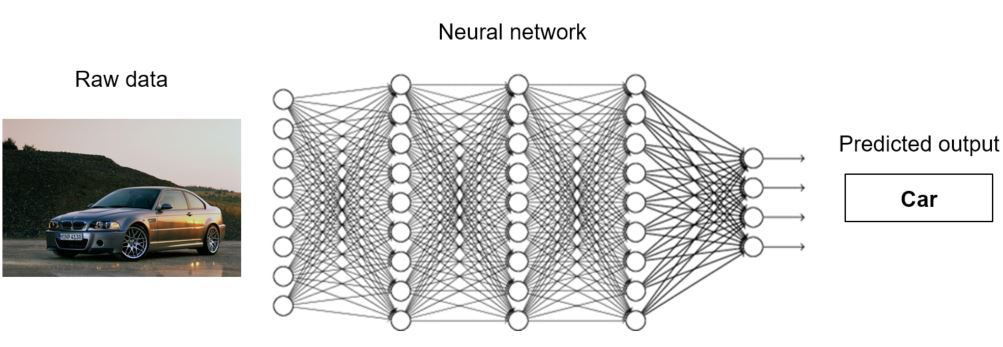
\includegraphics[width=1\textwidth]{nn}
	\caption{Jednoduchá architektúra NN s 1 vstupnou, 3 skrytími a 1 výstupou vrstvou\cite{odkaz:CorrectionOfImageOrentation}}
	\label{pic:NNExample}
\end{figure}

\subsubsection{Perceptron}
Pre pochopenie fungovania neurónovej siete je potrebné najprv pochopiť umelý neurón, zvaný perceptron.
Perceptron vynašiel vedec Frank Rosenblatt v 1950 až 1960 roku, inšpirovaný predchádzajucov prácov Warren McCulloch a Walter Pitts.
Dnes sa bežné používa iný model umelého neurónu tzv. sigmoid neurón\cite{odkaz:HandwrittenDigitRecognision}.

V jednoduchosti, perceptron zoberie niekoľko vstupov, $x_1, x_2, \dots$ a reprodukuje ich na jediný binárny výstup.
\begin{figure}[H]
	\centering
	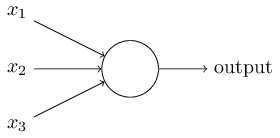
\includegraphics[width=0.4\textwidth]{tikz0}
	\caption{Jednoduchý príklad perceptronu\cite{odkaz:HandwrittenDigitRecognision}}
	\label{pic:Perceptron}
\end{figure}
Rosenblatt navrhol jednoduché pravidlo pre výpočet výstupu.
Zaviedol váhy[eng. weights], $w_1, w_2, \dots$,
    reálne čisla ktoré vyjadrujú dôležitosť príslušných vstupov vzhľadom na výstupy.
Výstup neurónu, 0 alebo 1, sa určuje podľa toho či vážena suma $\sum_j w_j x_j$ je menšia alebo väčsia ako určitá prahová hodnota.
Matematické vyjadrenie aktivačnej funkcie perceptronu by potom bolo\cite{odkaz:HandwrittenDigitRecognision}:
\begin{equation}
    output = 0, \; ak \; \sum_j w_j x_j \leq threshold
\end{equation}
\begin{equation}
    output = 1, \; ak \; \sum_j w_j x_j > threshold
\end{equation}

Matematický model perceptronu je možné zjednodušiť a to prepísaním formuly $\sum_j w_j x_j$ na skalárny súčin[eng. dot product],
    $w*x \equiv \sum_j w_j x_j$, kde $w$ a $x$ sú vektory váh a vstupov.
Druhá zmena je presun prahovej hodnoty na opačnú stranu nerovnice, a nahradiť ju tzv. perceptron bias, $b \equiv -threshold$.
Použitím týchto úprav bude model vyzerať nasledovne\cite{odkaz:HandwrittenDigitRecognision}:
\begin{equation}
    output = 0, \; ak \; w*x + b \leq 0
\end{equation}
\begin{equation}
    output = 1, \; ak \; w*x + b > 0
\end{equation}

\begin{figure}[H]
    \centering
    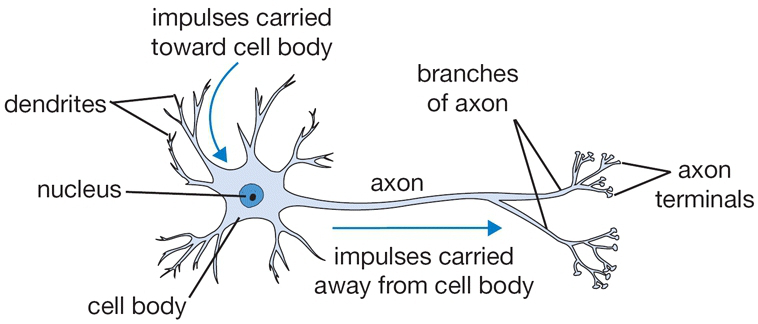
\includegraphics[width=0.5\textwidth]{neuron}
    \qquad
    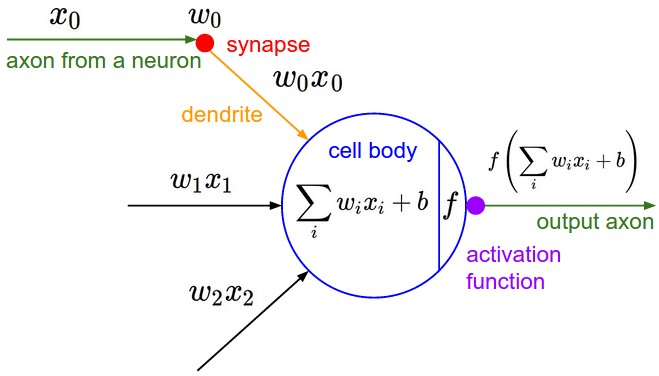
\includegraphics[width=0.4\textwidth]{neuron_model}
    \caption{biologický neurón(vľavo) a jeho matematický model(vpravo)\cite{odkaz:ConvolutionalNeuralNetworkCS231n}}
    \label{pic:Neuron}
\end{figure}

\subsubsection{Sigmoid}
Sigmoid je jedna z aktivačných funkcií používana v neurónových sietach, jej matematická formula je
\begin{equation}
    \sigma(x) = \frac{1}{1 + e^{-x}}
\end{equation}
zobrazená na obrázku \ref{pic:ActivationFunctions} vľavo.

Funkcia zoberie skutočné číslo a ''stlačí'' ho do rozmedzia 0 až 1.
Kde veľké záporne čísla nadobudnú hodnotu 0 a veľke kladné čísla hodnotu 1.
Funkcia sigmoid sa historicky často používala pretože má peknú interpretáciu pre spúštanie ''výstrelu'' neurónu,
    od nevýpalanie (0) až po úplne nasýtenie strely pri predpokladanej maximálnej frekvancií (1).
V praxi, sa sigmoid používa už len zriedka.
Pretože ma 2 hlavné nevýhody\cite{odkaz:ConvolutionalNeuralNetworkCS231n}:
\begin{enumerate}
    \item[$\bullet$] \textbf{Zabíjanie gradientov} - keď sa aktivácia neurónu nasýti na obidvoch koncoch 0 alebo 1, gradient v týchto oblastiach je takmer nulový.
    Tento gradient sa používa pri spätnej propagácií[eng. backpropagation] v neurónových sietach. Preto ak je miestny gradient veľmi malý, takmer žiaden signál
    neurónom nepreteká k jeho váham a rekurzívne k jeho dátam. Rovnako ak pri inicializácií sú váhy príliš veľké, väčsina neurónov by bola nasýtených a sieť by sa sotva niečo učila.
    \item[$\bullet$] \textbf{Výstupy nie sú centrované na nulu} - to má dôsledky na dynamiku pri klesaní gradient-u, pretože ak sú údaje prichádzajúce do neurónu vždy kladné,
    potom gradient na váhach $w$ nadobudne, počas spätnej propagáciie, všetky hodnoty pozitívne alebo negatívne (v závisloti na gradient-e celého výrazu).
    To by mohlo viesť k nežiadúcej cik-cakovitej dynamike pri aktualizáciach gradient-ov pre váhy.
\end{enumerate}


\subsubsection{Tanh}
Funkcia tanh je dalšou z aktivačných funkcií neurónu je zobrazená na obrázku \ref{pic:ActivationFunctions} vpravo.
Tanh zoberie skutočné čislo a stlačí ho do rozmedzia -1 až 1. Pracuje podobne ako sigmoid.
Matematický zápis je\cite{odkaz:ConvolutionalNeuralNetworkCS231n}:
\begin{equation}
    tanh(x) = 2\sigma(2x) - 1
\end{equation}
Kedže netrpí nevýhodami ako sigmoid tak v praxi je preferovanejší.


\begin{figure}[H]
    \centering
    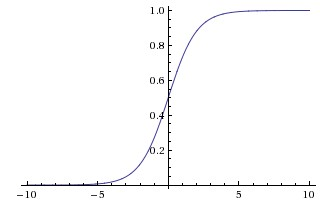
\includegraphics[width=0.45\textwidth]{sigmoid}
    \qquad
    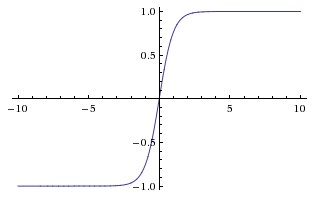
\includegraphics[width=0.45\textwidth]{tanh}
    \caption{
        Vľavo: Sigmoid nelineárne stlačenie čísel do rozsahu [0,1],
        Vpravo: Tanh nelineárne stlačenie čísel do rozsahu [-1,1] \cite{odkaz:ConvolutionalNeuralNetworkCS231n}
    }
    \label{pic:ActivationFunctions}
\end{figure}

\subsubsection{ReLU a Leaky ReLU}
V praxi existuje niekoľko dalšich aktivačných funkcií, každá je použitelná pre riešenie iného problému,
    čiže každá ma svoje výhody ale aj nevýhody.
Ako príklad môžeme uviesť ReLU (Rectified Linear Unit)
\begin{equation}
    f(x) = max(0,x)
\end{equation}
alebo jeho obdobu Leaky ReLU, ktorá sa snaží vyriešiť nevýhody ReLU.
\begin{equation}
    f(x) = x \quad ak \; x > 0
\end{equation}
\begin{equation}
    f(x) = ax \quad ak \; x <= 0
\end{equation}
kde $a$ je malá konštanta (napr. 0.01) \cite{odkaz:ConvolutionalNeuralNetworkCS231n}.

\subsubsection{Architektúra neurónovej siete}
Ako bolo spomínane už vyššie, neurónová sieť je modelovaná ako kolekcia neurónov, ktoré sú prepojené v acyklickom grafe.
Modely neurónových sieti sú často organizované do odlišných vrstiev neurónov.
Pre bežné neurónové siete je najbežnejšou vrstvou tzv. plne-prepojená vrstva [eng. fully-connected layer],
    v ktorej sú neuróny medzi dvoma priľahlými vrstvami plne párovo prepojené, ale neuróny v jeden vrstve nemajú medzi sebou žiadne spojenia.
Na obrázku \ref{pic:NeuralNetworkArchitecture} nižšie sú uvedené dve topológie ktoré využívajú plne-prepojené vrstvy\cite{odkaz:ConvolutionalNeuralNetworkCS231n}:
\begin{figure}[H]
    \centering
    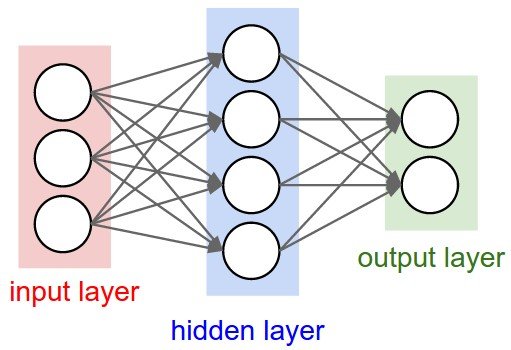
\includegraphics[width=0.38\textwidth]{neural_net}
    \qquad
    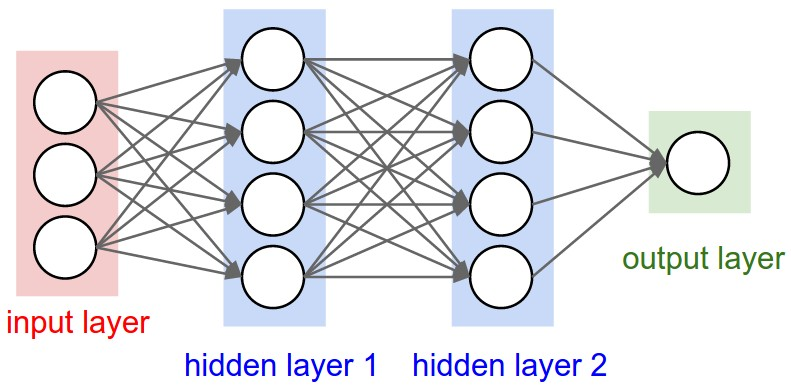
\includegraphics[width=0.52\textwidth]{neural_net2}
    \caption{Vľavo: 2-vrstvová neurónová sieť, Vpravo: 3-vrstvová neurónová sieť \cite{odkaz:ConvolutionalNeuralNetworkCS231n}}
    \label{pic:NeuralNetworkArchitecture}
\end{figure}

Vačšie neurónové sieťe dokážu reprezentovať komplikovanejšie funkcie.
Na obrázku \ref{pic:XNNLayerExample} je vidieť rozdiel klasifikácie dát do 2 tried (červená, zelená) použitím rôznych veľkostí neurónových sieti.
\begin{figure}[H]
	\centering
	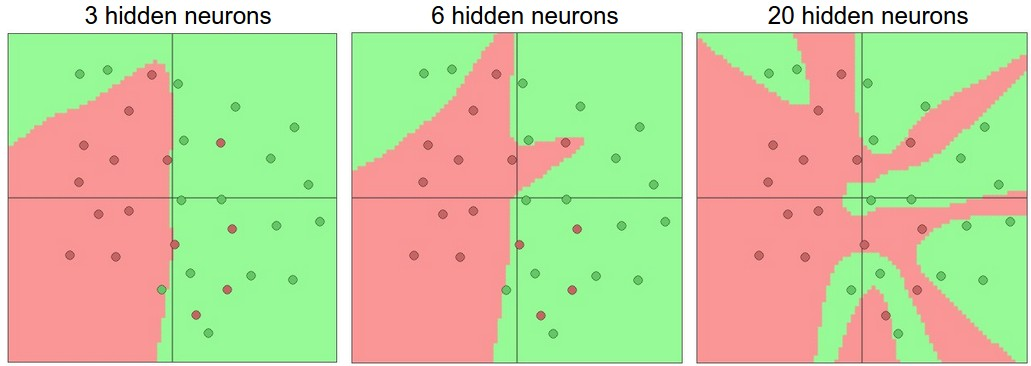
\includegraphics[width=1\textwidth]{layer_sizes}
	\caption{Zobrazenie klasifikácie dát rôznymi veľkostami NN \cite{odkaz:ConvolutionalNeuralNetworkCS231n}}
	\label{pic:XNNLayerExample}
\end{figure}

\subsection{Konvolučné neurónové siete}
Konvolučné neurónové siete [eng. convolutional neural networks] (CNNs), sú špeciálnym prípadom neurónových sieti pre spracovanie
    dát, ktoré majú známu topológiu podobnú mriežke.
Pre príklad je možné uviesť 2-dimenzionálne dáta ako sieť pixelov pri spracovaní obrázkov.
Názov týchto sieti \textit{konvolučné} indikuje používanie matematickej operácie zvanej konvolúcia[eng. convolution]\cite{book:Goodfellow-et-al-2016}.

\subsubsection{Konvolúcia}
Vo svojej najvšeobecnejšej podobe, konvolúcia je operácia dvoch funkcií s reálnymi hodnotami argumentov.
Operácia konvolúcie je typicky označovaná hviezdičkou:
\begin{equation}
    s(t) = (x * w)(t)
\end{equation}
V terminilógií konvolučnej siete je prvý argument (v tomto príklade funkcie $x$) sa často označuje ako vstup a druhý
    argument (v tomto príklade funkcia $w$) ako jadro[eng. kernel]. Výstup je niekedy označovaný ako mapa príznakov.

Bežne konvolúciu používame na viac ako jednej osy súčasne.
Pri použítí 2-dimenzionálneho obrázku $I$ ako náš vstup, budeme chcieť použiť aj 2-dimenzionálne jadro $K$\cite{book:Goodfellow-et-al-2016}:
\begin{equation}
    S(i,j) = (I * K)(i, j) = \sum_m \sum_n I(m,n) K(i - m, j - n)
\end{equation}

Avšak množstvo knižníc, ktoré implementujú neurónové siete, používajú tzv. cross-correlation funkciu\cite{book:Goodfellow-et-al-2016}:
\begin{equation}
    S(i,j) = (I * K)(i, j) = \sum_m \sum_n I(i + m, i + n) K(m, n)
\end{equation}

\subsubsection{Architektúra}
CNN využívajú skutočnosti, že vstup pozostáva z obrázkov.
Na rozdiel od obyčajnej neurónovej siete majú vrstvy CNN neuróny usporiadané v troch rozmeroch: šírka, výška, hĺbka[eng. width, height, depth].
Hĺbka odkazuje na 3.dimenziu aktivačného zväzku[eng. activation volume], nie na celkovú hĺbku neurónovej siete.
Neuróny vo vrtsve budú prepojené iba k malej oblasti vrstvy pred ňou, namiesto plného prepojenia \cite{odkaz:CNNArchitecture}.

Pre stavbu CNN sa využívajú 3 základne typy vrstiev:
\begin{enumerate}
    \item[$\bullet$] \textbf{Convolutional layer} - konvolučná vrstva je hlavný stavebný blok CNN, ktorá vykonáva väčšinu výpočtov.
    Parametre tejto vrstvy pozostávajú zo súboru filtrov, ktoré sa dokážu učiť.
    Takto naučené filtre sa aktivujú keď uvidia určitý typ vizuálneho prvku, napr. hranu určitej orientácie alebo škvrnu určitej farby a pod..
    \item[$\bullet$] \textbf{Pooling layer} - táto vrstva je obvykle vkladaná ako spojenie medzi dvoma konvolučnímy vrstvami.
    Jej funkciou je postupné znižovanie priestorovej veľkosti reprezentovaného vstupu, pre zníženie množstva parametrov a výpočtov v sieti, a teda aj kontroly pretrénovania.
    \item[$\bullet$] \textbf{Fully-Connected layer} - rovnako ako v obvyklých neurónových sietach, je to vrstva kde všetky neuróny sú prepojené s predchádzajucou vrstvou.
\end{enumerate}

\begin{figure}[H]
	\centering
	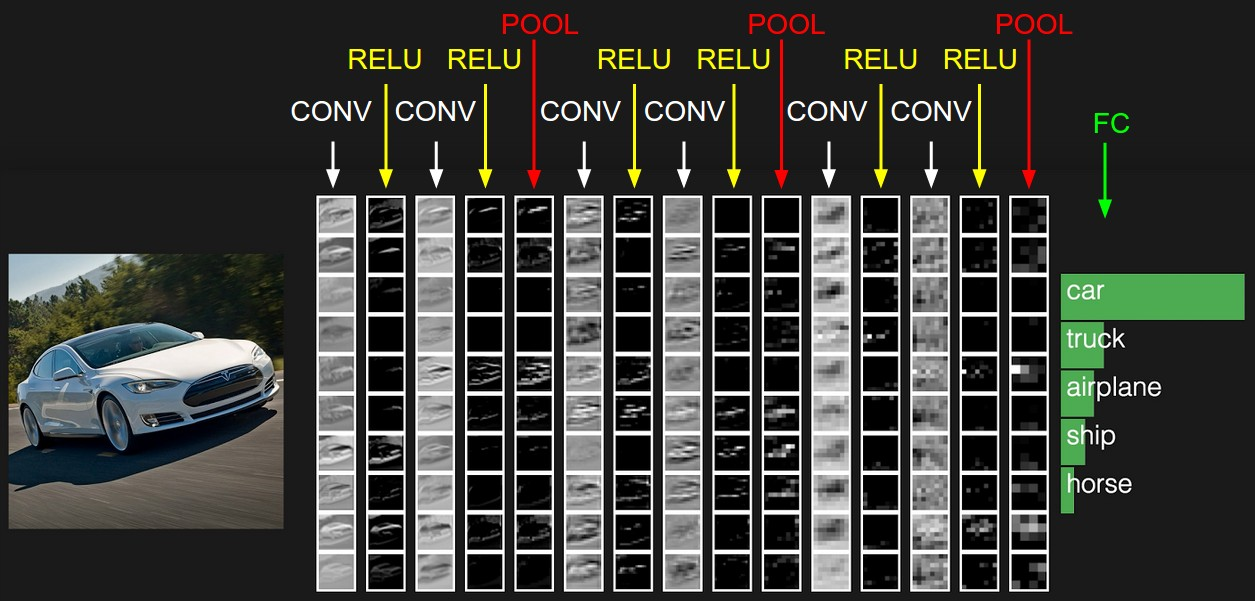
\includegraphics[width=1\textwidth]{convnet}
	\caption{Príklad architektúry konvolučnej neurónovej siete \cite{odkaz:CNNArchitecture}}
	\label{pic:CNNExample}
\end{figure}
